\documentclass[12pt]{article}
\usepackage{common}
% \usepackage{todonotes}
% \usepackage[nomarkers]{endfloat}
\linespread{1.25}
% \usepackage{silence}
% \WarningFilter{latex}{Text page}

\usepackage[pdftex,
            pdfauthor={Richard Ouyang},
            pdftitle={Predicting LendingClub Loan Repayments and Interest Rates},
            colorlinks=true]{hyperref}

\title{Predicting LendingClub Loan Repayments and Interest Rates}
\author{Richard Ouyang}
\date{May 5, 2018}

\begin{document}

\maketitle

\begin{abstract}
Using a dataset of loans issued from 2007--2011 by LendingClub, a peer-to-peer lending company, I use several machine-learning techniques to predict whether a given loan was eventually fully paid off as well as the interest rate chosen by LendingClub for the loan. I find that ensemble tree models, particularly gradient-boosted trees, perform significantly better than the standard logistic and linear models for classification and regression, respectively. Feature importances of these tree models as well as significance tests in logistic and linear regressions are consistent with prior intuition on both loan repayment and interest rates. Borrower characteristics that reflect a long credit history or sound financial responsibility, such as low revolving utilization, are positively associated with loan repayment probability and negatively associated with interest rate, which is consistent with intuition. Additionally, loan size and using the loan for small business purposes have the opposite effect.
\end{abstract}

\newpage
\tableofcontents

\newpage
\section{Introduction}

\subsection{LendingClub}

LendingClub \cite{lendingclub} is a peer-to-peer lending company in which individual investors can buy securities backed by payments made by borrowers of personal loans. Borrowers can obtain unsecured personal loans ranging in value from \$1,000 to \$40,000. After borrowers submit information on their credit history and the purpose for the loan application, LendingClub chooses whether to accept or reject the loan, assigning it a grade, subgrade, and interest rate in the former case. Individual investors can then receive exposure to consumer credit either by selecting a strategy that chooses loans based on credit risk or by manually choosing which loans in which to invest. Origination fees from borrowers and service fees from investors make up LendingClub's revenue.

% As a result, LendingClub has an incentive to accept only loans which it believes investors will find attractive. 

\subsection{Prediction}

Credit (default) risk is perhaps the most important factor when considering the value of a loan \cite{diette2000how}. Therefore, in addition to the interest rate, one of the main factors in choosing loans in which to invest is the probability that the borrower will fully pay off the loan. As a result, a model that accurately predicts the probability of full repayment is useful to an investor seeking more accurate estimates of loan values. This paper seeks to use data on past loans in order to create a predictive model of loan repayment. 

Another section of the consumer credit space in which predictive algorithms are helpful is in the prediction of the interest rate a particular loan application will receive. With such algorithms and information, potential investors and borrowers can understand how LendingClub and other lenders consider borrower and loan characteristics -- as well as their interactions between variables -- when processing loan applications; therefore, investors and borrowers can make more informed decisions about their investments and loans. To this end, this paper seeks to develop a model for predicting the interest rate chosen by LendingClub given only information known at the time of the loan application. 

\subsection{Machine Learning Models for Classification and Prediction}

Perhaps the most common methods used for classification and prediction in economics are logistic and linear regression \cite{menard2018applied}. Regression techniques have the advantage of being able to accommodate causal inference, but in prediction settings such as the ones discussed in this paper, machine learning techniques have become far more popular. In particular, two general methods discussed in lecture are neural networks and tree models. I will briefly describe in more detail three types of tree models, and more information about neural networks is available at \cite{haykin2004neural}.

\subsubsection{Tree Models}

The random forest \cite{breiman2001random} is a type of tree model in which many decision trees are constructed (as described in lecture). Each decision tree is constructed by randomly selecting elements of the original dataset with replacement, and the tree is grown using a random subset of the features. At each node, the best possible split of variables is chosen until the tree is fully grown. Although each decision tree has very high variance, a low correlation between each tree allows a large number of trees to reduce the variance of the predictor and thus increase its accuracy. In order to predict an outcome given the feature variables, each decision tree in the random forest gives its prediction. For classification, the predicted probability that the input is in class $c$ is the proportion of trees that predict class $c$; for regression, the predicted value for the whole random forest is the average prediction over all decision trees.

Despite being a relatively simple method, several features of the random forest make it extremely effective. Unlike many other statistical techniques, random forests do not suffer from overfitting because adding trees to the forest merely reduces variance. Additionally, it nicely handles variable selection because at each point in the decision tree, the algorithm chooses the most discriminative variable split, therefore implicitly choosing the most important features. In contrast, most econometric regression techniques require careful variable selection and use of significance tests. Moreover, because the model is trained based on splits of the data rather than absolute values, the random forest is robust to one-to-one transformations, such as constant multiplication or squaring of non-negative values, of feature variables and thus does not need robustness checks via varying specifications or encodings of sequential or ordinal feature variables. 

Extremely randomized trees \cite{geurts2006extremely} offer a slight variant on random forests in which a random split (based on the empirical range of the variable in question), rather than the best split, is chosen at each point in the decision tree. 

Yet another alternative is gradient tree boosting \cite{chen2016xgboost}, an iterative algorithm in which at each step, the most recent, imperfect decision tree $F_t$ is improved to $F_{t+1}$ by adding another decision tree $h_t$ which is trained on the residual of $F_t$. The predictor is repeatedly improved in this manner for a fixed number of iterations.   

% \subsubsection{Neural Networks}

% Neural networks, as discussed in lecture, are another common method of prediction. \cite{haykin2004neural}\todo{either talk more about neural nets or delete this}

\section{Data}

The dataset used in this paper contains information on 42,538 loans approved by LendingClub from 2007--2011 and was obtained from \cite{lendingclub}. After cleaning the dataset, each loan contains the information in Table \ref{table:variables}. After omitting loans in which more than 30\% of the variables were missing, the final, clean dataset contained 42,506 loans.

\begin{table}[!ht]
\footnotesize
\centering

\begin{tabular}{p{5cm}p{10cm}}
\toprule
\textbf{Variable name} & \textbf{Description} \\ \midrule
\texttt{funded\_amount} & The total amount committed to the loan \\
\texttt{term} & The number of payments on the loan. Values are in months and can be either 36 or 60. \\
\texttt{interest\_rate} & Interest rate on the loan \\
\texttt{installment} & The monthly payment owed by the borrower \\
\texttt{grade} \& \texttt{subgrade} & LendingClub-assigned loan (sub)grade, a measure of credit risk \\
\texttt{employment\_length} & Employment length in years. Possible values are between 0 and 10 where 0 means less than one year and 10 means ten or more years. \\
\texttt{home\_ownership} & The home ownership status provided by the borrower during registration. Values are: RENT, OWN, MORTGAGE, OTHER. \\
\texttt{annual\_income} & The self-reported annual income provided by the borrower \\ 
\texttt{verification\_status} & Whether income was verified by LendingClub \\
\texttt{issue\_date} & The month in which the loan was funded \\
\texttt{purpose} & A category provided by the borrower for the loan request \\
\texttt{address\_state} & The state provided by the borrower \\
\texttt{dti} & The borrower's total monthly debt payments (excluding mortgages) divided by the borrower's self-reported monthly income. \\
\texttt{delinq\_2yrs} & The delinquencies in the past 2 years \\
\texttt{earliest\_credit\_line} & The month in which the borrower's earliest reported credit line was opened \\
\texttt{inquiries\_last\_6months} & The number of inquiries in the past 6 months, excluding auto and mortgage inquiries \\
\texttt{open\_accounts} & The number of open credit lines in the borrower's credit file \\
\texttt{pub\_rec} & Number of derogatory public records \\
\texttt{revolving\_balance} & Total credit revolving balance \\
\texttt{revolving\_utilization} & Revolving line utilization rate \\
\texttt{total\_accounts} & The total number of credit lines currently in the borrower's credit file \\
\texttt{pub\_rec\_bankruptcies} & Number of public record bankruptcies \\
\texttt{tax\_liens} & Number of tax liens \\

\bottomrule
\end{tabular}
\caption{Variables included in the dataset. Some variables were omitted if either no values for that variable were available, every loan in the dataset had the same value for that variable, or the variable became known only after the loan had originated. Data from \cite{lendingclub}.}
\label{table:variables}
\end{table}

First, I attempt to predict whether the loan was fully paid or charged off, given only information known at the start of the loan (all such variables make up Table \ref{table:variables}). Additionally, I also attempt to predict LendingClub's interest rate for the loan given only information known when the borrower applied for the loan. In this particular case, I use all of the variables in Table \ref{table:variables} except the interest rate, the installment amount, the loan grade, and the loan subgrade to predict LendingClub's chosen interest rate. Therefore, if sufficiently predictive, this algorithm approximates LendingClub's own interest-rate determination algorithm and provides insight into what LendingClub considers before originating loans. 

\section{Methods}

I used Python for all coding portions of the project. In particular, I used the Python packages \texttt{scikit-learn} \cite{pedregosa2011scikit} and \texttt{statsmodels} \cite{seabold2010statsmodels}. For each of the two prediction settings (predicting repayment and interest rate), I used simple regression techniques, neural networks, and the three tree models described above. The code used to clean the data and generate the results and visualizations is available in Appendix \ref{appendix:code}.

% \todo{maybe start with a subsection about logistic regression}

\subsection{Hyperparameter Tuning}

Although linear and logistic regression require little or no parameter tuning outside variable selection (regularization parameters are sometimes needed), tree models have several parameters that may require tuning. The most important parameter is the number of decision trees included in the model; increasing the number of decision trees reduces the variance and improves the accuracy of the model \cite{breiman2001random}. Other major parameters for tree models include the number of features (usually a subset of the total number of features) to consider at each split, the maximum depth of each decision tree, and the acceptable size range for each leaf in the tree \cite{pedregosa2011scikit}. Additional parameters for gradient tree boosting include the learning rate (how quickly and finely the tree learns) \cite{chen2016xgboost}. In developing the final model for the two prediction settings, I will experiment with several values of each of these parameters in order to improve the out-of-the-box model.

\subsection{Classification Evaluation}

I trained each model on a random 70\% of the data and obtained a generalization error using the other 30\%. For classification, I consider the accuracy rate (number of correct guesses divided by the total number of guesses). I also compute the receiver operating characteristic (ROC) curve \cite{bradley1997use}. The ROC curve plots the false positive rate ($x$-axis) against the true positive rate, also known as the sensitivity ($y$-axis), therefore visualizing the tradeoff between the two. As such, the ROC AUC score, which is the area under the ROC curve, corresponds to the probability that a randomly chosen positive data point will have a higher predicted probability than a randomly chosen negative data point. The AUC score is typically a better measure of the accuracy of a predictive model, and the higher the score, the better \cite{bradley1997use}.

Another measure of the accuracy of a classification model is the log-likelihood, calculated for loan $i$ as $(1 - y_i)\log(1 - \hat{p}_i) + y_i\log \hat{p}_i$, where $y_i$ is the indicator of whether loan $i$ is in a particular class (i.e., was ultimately fully paid), and $\hat{p}_i$ is the probability predicted by the model that loan $i$ is in the predicted class. Better models have higher values for the log-likelihood. 

Yet another measure of classification accuracy is the Brier score, computed as the mean square difference between the predicted probability and the class indicator for loan $i$. Smaller Brier scores imply better models.

% \todo{Also the confusion matrix (see where the classifier goes wrong)}

\subsection{Regression Evaluation}

The main measures of accuracy when evaluating regression models are $R^2$, which is the fraction of the variance in the data explained by the model (or alternatively, the square of the correlation between the model's predictions and the true values), and the mean square error (MSE) and mean absolute error (MAE), which are the mean squared (or absolute) difference between the model's predictions and the true value. 

\section{Results and Discussion}

\subsection{Classification}
\label{subsection:classification_results}

Since logistic regression is the standard for econometric analysis, I first present the output from fitting a logit model to predict loan repayment. The output for the logistic regression is at Table \ref{table:logistic_results}. 

There were several major factors that negatively affected the probability that a given loan was repaid. Since both \texttt{term} and \texttt{interest\_rate} are positively correlated with the size of the loan, the decrease in loan repayment probability associated with increases in these features is consistent with intuition since larger loan sizes typically correspond to lower repayment probability. \texttt{inquiries\_last\_6months}, \texttt{revolving\_balance}, and \texttt{revolving\_utilization} are all negatively associated with good credit and financial responsibility, so the coefficients of these variables are also consistent with intuition. The negative coefficient on \texttt{purpose\_small\_business} suggests that people who use LendingClub for small business funding are less likely to repay the loan than on average, adjusting for other factors. One possible interpretation of this coefficient is that successful small business owners typically do not need to reach out to LendingClub for loans; outside investors can either invest in equity or buy loans via banks. Alternatively, since small businesses are generally likely to fail, borrowers are much less likely to repay loans created to sustain such businesses.

On the other hand, the variable that most significantly (by far) increases a given loan's repayment probability is \texttt{annual\_income}. This suggests that increases in annual income correspond to higher loan repayment probabilities, an assertion that is also consistent with intuition and prior knowledge. 

\begin{table}[!htbp]
    \footnotesize
    \begin{center}
\begin{tabular}{lclc}
\toprule
\textbf{Dep. Variable:}                        &   loan\_status    & \textbf{  No. Observations:  } &    29754    \\
\textbf{Model:}                                &      Logit       & \textbf{  Df Residuals:      } &    29712    \\
\textbf{Method:}                               &       MLE        & \textbf{  Df Model:          } &       41    \\
\textbf{Date:}                                 & Sun, 04 Mar 2018 & \textbf{  Pseudo R-squ.:     } &  0.07905    \\
\textbf{Time:}                                 &     14:08:21     & \textbf{  Log-Likelihood:    } &   -11667.   \\
\textbf{converged:}                            &       True       & \textbf{  LL-Null:           } &   -12669.   \\
\bottomrule
\end{tabular}
\begin{tabular}{lcccccc}
                                               & \textbf{coef} & \textbf{std err} & \textbf{z} & \textbf{P$>|z|$} & \textbf{[0.025} & \textbf{0.975]}  \\
\midrule
\textbf{funded\_amnt}                          &   -1.493e-05  &      1.5e-05     &    -0.995  &         0.320        &    -4.43e-05    &     1.45e-05     \\
\textbf{term}                                  &      -0.0194  &        0.003     &    -5.856  &         0.000        &       -0.026    &       -0.013     \\
\textbf{int\_rate}                             &      -0.1161  &        0.017     &    -6.763  &         0.000        &       -0.150    &       -0.082     \\
\textbf{installment}                           &       0.0004  &        0.001     &     0.881  &         0.378        &       -0.001    &        0.001     \\
\textbf{grade}                                 &       0.0413  &        0.124     &     0.333  &         0.739        &       -0.202    &        0.284     \\
\textbf{sub\_grade}                            &      -0.0199  &        0.140     &    -0.143  &         0.887        &       -0.294    &        0.254     \\
\textbf{emp\_length}                           &      -0.0123  &        0.005     &    -2.472  &         0.013        &       -0.022    &       -0.003     \\
\textbf{annual\_inc}                           &    7.156e-06  &     6.12e-07     &    11.701  &         0.000        &     5.96e-06    &     8.35e-06     \\
\textbf{dti}                                   &      -0.0011  &        0.003     &    -0.383  &         0.702        &       -0.007    &        0.005     \\
\textbf{delinq\_2yrs}                          &       0.0064  &        0.032     &     0.198  &         0.843        &       -0.057    &        0.070     \\
\textbf{inq\_last\_6mths}                      &      -0.1277  &        0.010     &   -12.246  &         0.000        &       -0.148    &       -0.107     \\
\textbf{open\_acc}                             &      -0.0066  &        0.005     &    -1.233  &         0.217        &       -0.017    &        0.004     \\
\textbf{pub\_rec}                              &      -0.1194  &        0.103     &    -1.164  &         0.245        &       -0.320    &        0.082     \\
\textbf{revol\_bal}                            &   -4.367e-06  &     9.02e-07     &    -4.841  &         0.000        &    -6.13e-06    &     -2.6e-06     \\
\textbf{revol\_util}                           &      -0.0041  &        0.001     &    -5.332  &         0.000        &       -0.006    &       -0.003     \\
\textbf{total\_acc}                            &       0.0019  &        0.002     &     0.811  &         0.417        &       -0.003    &        0.006     \\
\textbf{pub\_rec\_bankruptcies}                &      -0.2095  &        0.122     &    -1.711  &         0.087        &       -0.450    &        0.030     \\
\textbf{tax\_liens}                            &      34.0041  &     3.36e+07     &  1.01e-06  &         1.000        &    -6.58e+07    &     6.58e+07     \\
\textbf{has\_employment}                       &       0.7333  &        5.817     &     0.126  &         0.900        &      -10.667    &       12.133     \\
\textbf{issue\_month}                          &       0.0002  &        0.005     &     0.041  &         0.968        &       -0.010    &        0.010     \\
\textbf{issue\_year}                           &       0.1063  &        0.023     &     4.665  &         0.000        &        0.062    &        0.151     \\
\textbf{earliest\_cr\_line\_month}             &       0.0179  &        0.005     &     3.784  &         0.000        &        0.009    &        0.027     \\
\textbf{earliest\_cr\_line\_year}              &       0.0013  &        0.003     &     0.435  &         0.663        &       -0.004    &        0.007     \\
\textbf{home\_ownership\_NONE}                 &      -0.8326  &        1.206     &    -0.691  &         0.490        &       -3.196    &        1.531     \\
\textbf{home\_ownership\_OTHER}                &      -0.4725  &        0.248     &    -1.906  &         0.057        &       -0.958    &        0.013     \\
\textbf{home\_ownership\_OWN}                  &      -0.0387  &        0.067     &    -0.574  &         0.566        &       -0.171    &        0.094     \\
\textbf{home\_ownership\_RENT}                 &      -0.0499  &        0.040     &    -1.247  &         0.212        &       -0.128    &        0.029     \\
\textbf{purpose\_credit\_card}                 &      -0.0419  &        0.118     &    -0.355  &         0.723        &       -0.273    &        0.189     \\
\textbf{purpose\_debt\_consolidation}          &      -0.2863  &        0.109     &    -2.638  &         0.008        &       -0.499    &       -0.074     \\
\textbf{purpose\_educational}                  &      -0.6269  &        0.183     &    -3.434  &         0.001        &       -0.985    &       -0.269     \\
\textbf{purpose\_home\_improvement}            &      -0.3275  &        0.123     &    -2.659  &         0.008        &       -0.569    &       -0.086     \\
\textbf{purpose\_house}                        &      -0.3942  &        0.193     &    -2.042  &         0.041        &       -0.772    &       -0.016     \\
\textbf{purpose\_major\_purchase}              &      -0.1207  &        0.134     &    -0.904  &         0.366        &       -0.382    &        0.141     \\
\textbf{purpose\_medical}                      &      -0.5743  &        0.158     &    -3.640  &         0.000        &       -0.883    &       -0.265     \\
\textbf{purpose\_moving}                       &      -0.6451  &        0.165     &    -3.910  &         0.000        &       -0.968    &       -0.322     \\
\textbf{purpose\_other}                        &      -0.5334  &        0.115     &    -4.618  &         0.000        &       -0.760    &       -0.307     \\
\textbf{purpose\_renewable\_energy}            &      -0.6564  &        0.347     &    -1.890  &         0.059        &       -1.337    &        0.024     \\
\textbf{purpose\_small\_business}              &      -1.0789  &        0.123     &    -8.791  &         0.000        &       -1.319    &       -0.838     \\
\textbf{purpose\_vacation}                     &      -0.5716  &        0.203     &    -2.810  &         0.005        &       -0.970    &       -0.173     \\
\textbf{purpose\_wedding}                      &      -0.1158  &        0.162     &    -0.715  &         0.475        &       -0.433    &        0.202     \\
\textbf{verification\_status\_Source Verified} &      -0.0177  &        0.046     &    -0.382  &         0.703        &       -0.109    &        0.073     \\
\textbf{verification\_status\_Verified}        &      -0.0243  &        0.045     &    -0.545  &         0.586        &       -0.112    &        0.063     \\
\bottomrule
\end{tabular}
% \caption{Logit Regression Results}
\end{center}
    \caption{Logistic regression results.}
    \label{table:logistic_results}
\end{table}

Figures \ref{fig:calibration}, \ref{fig:prob_hist}, \ref{fig:roc_curve}, \ref{fig:auc}, \ref{fig:brier}, and \ref{fig:log_likelihood} have several visualizations of the classification models used in this paper. Gradient tree boosting (XGBoost) was consistently the best model by all accuracy metrics considered, and the logistic regression and neural network had the worst predictive power. The AUC score, the Brier score, and the log-likelihood all resulted in the same ordering of the candidate models in terms of accuracy.

From the calibration curve in Figure \ref{fig:calibration}, it is clear that most models had very good calibration for fully-paid loans but performed worse on more risky loans. In particular, when the predicted probabilities of loan repayment outputted by the models fall below about $0.4$, the calibration curve begins to deviate significantly from the dotted line, which represents perfect calibration. Additionally, while most of the tree models were relatively well-calibrated for high probabilities of loan repayment, the logistic model consistently overestimated the actual probability of loan repayment, as evidenced by the fact that the logistic calibration curve is consistently below the dotted line. The neural network calibration curve also exhibits some peculiarities in that it's remarkably horizontal. This suggests that the neural network's predicted probabilities are not very effective relative to the other models. 

Pecularities with the neural network are also evident in the ROC curve (Figure \ref{fig:roc_curve}) in that its curve is much lower than even the logistic curve. Again, this suggests that the neural network's predicted probabilities are ineffective. 

In order to improve accuracy, I opted to add yet another classification model, one that averages (weighted by each original model's accuracy) the predicted probabilities of the two best individual models, the random forest and gradient tree boosting, to produce a new predicted probability. This voting classifier, as shown in Figures \ref{fig:roc_curve}, \ref{fig:auc}, \ref{fig:brier}, and \ref{fig:log_likelihood}, shows slightly better results across all accuracy metrics than any individual model. 

\begin{figure}[!htbp]
    \centering
    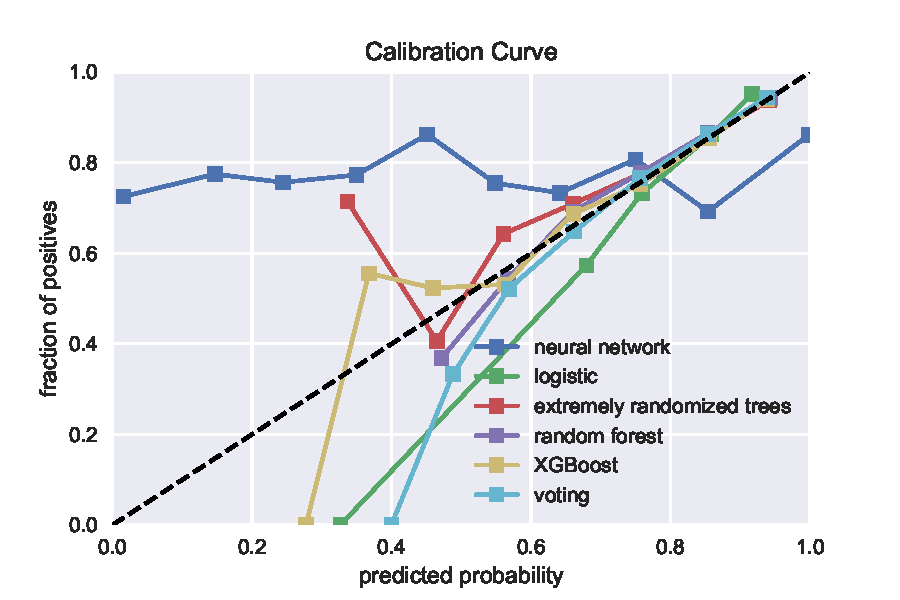
\includegraphics[width=\textwidth]{graphics/calibration_curve}
    \caption{Calibration curve for classification models. A curve closer to the dotted line corresponds to a more calibrated (predicted probabilities are consistent with empirical probabilities) model.}
    \label{fig:calibration}
\end{figure}

\begin{figure}[!htbp]
    \centering
    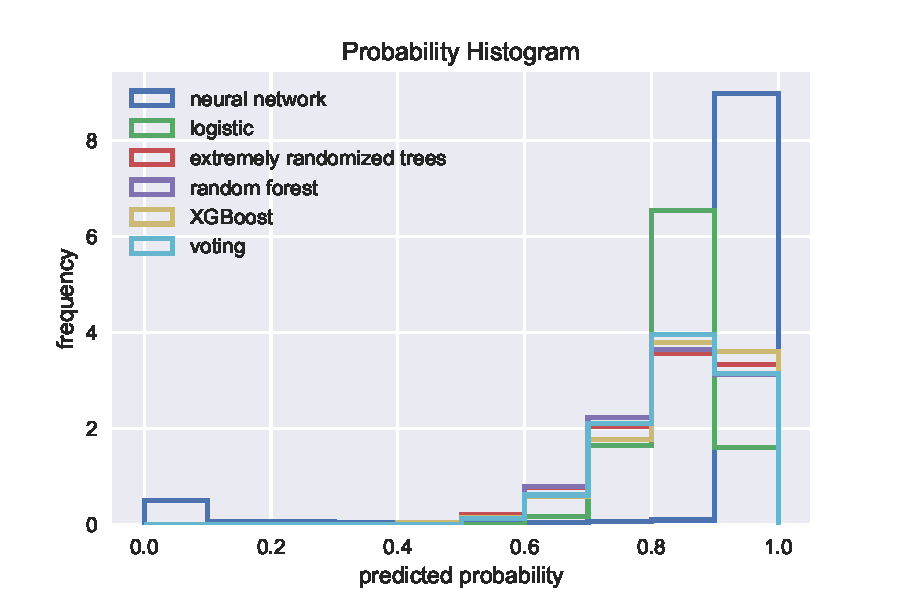
\includegraphics[width=\textwidth]{graphics/prob_hist}
    \caption{Predicted probability histogram for classification models.}
    \label{fig:prob_hist}
\end{figure}

\begin{figure}[!htbp]
    \centering
    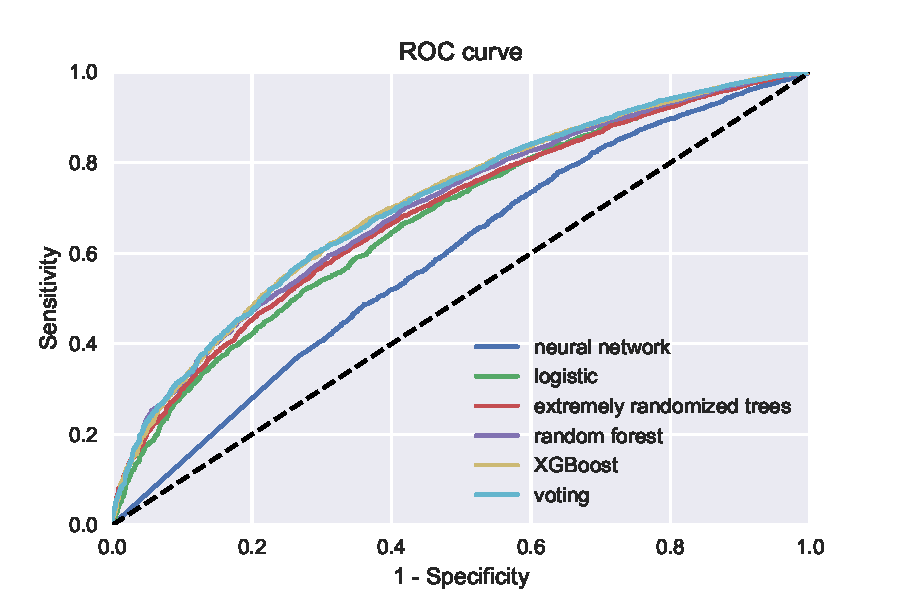
\includegraphics[width=\textwidth]{graphics/roc_curve}
    \caption{ROC curve for classification models. A higher ROC curve (farther from the dotted line) corresponds to a better model.}
    \label{fig:roc_curve}
\end{figure}

\begin{figure}[!htbp]
    \centering
    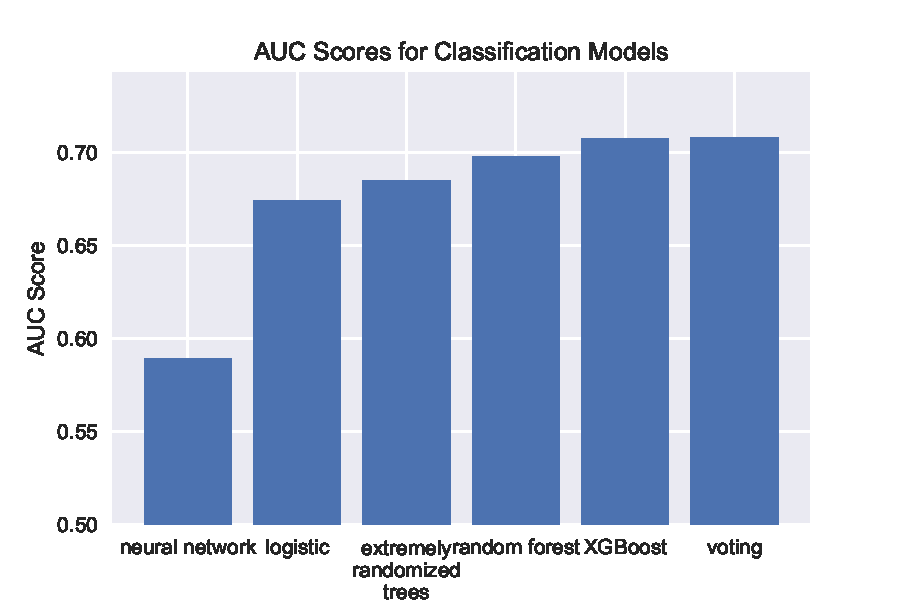
\includegraphics[width=\textwidth]{graphics/classification_auc}
    \caption{AUC score comparison for classification models. A higher AUC score corresponds to a better model.}
    \label{fig:auc}
\end{figure}

\begin{figure}[!htbp]
    \centering
    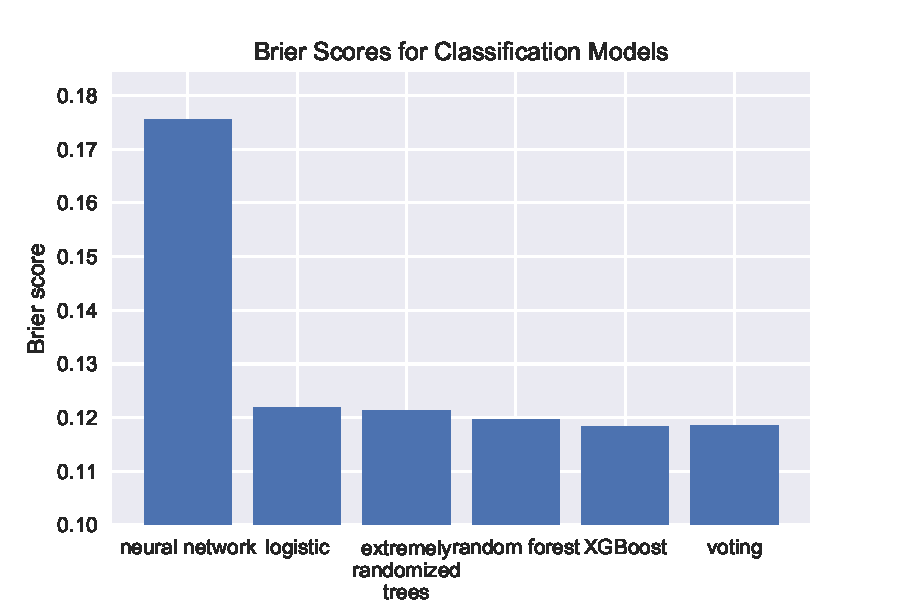
\includegraphics[width=\textwidth]{graphics/classification_brier}
    \caption{Brier score comparison for classification models. A lower Brier score corresponds to a better model, with $0$ corresponding to a perfect model and $1$ corresponding to a random model.}
    \label{fig:brier}
\end{figure}

\begin{figure}[!htbp]
    \centering
    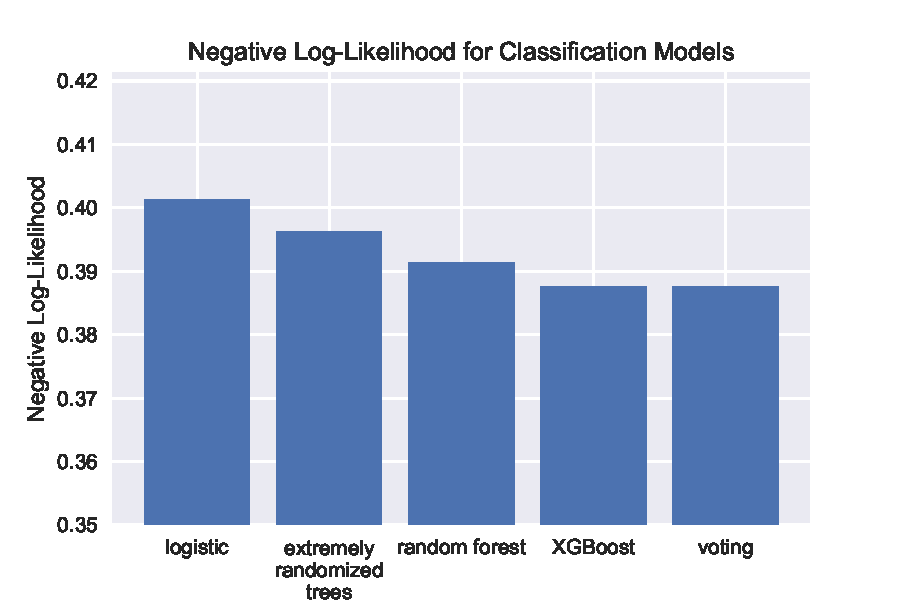
\includegraphics[width=\textwidth]{graphics/classification_loglik}
    \caption{Negative log-likelihood for classification models. The neural network was not included since its log-likelihood was not finite. A lower negative log-likelihood corresponds to a better model.}
    \label{fig:log_likelihood}
\end{figure}

% \subsubsection{Accuracy Rates}

% Table with best result for each method

% It is often difficult for algorithms to classify heavily imbalanced data \cite{chen2004using}. The LendingClub dataset, which consists of approximately 85\% fully paid loans, exhibits this problem as well, since without careful hyperparameter tuning, some algorithms classify every single data point as the larger class. 

% Several methods -- for example, using balanced or weighted versions of tree models like random forests \cite{chen2004using} -- have been proposed as fixes for imbalanced data. 

% \todo{a table consisting of the AUC scores for each method}

% \todo{confusion matrix} 

\subsubsection{Feature Importances}

One nice property of tree models is that they provide a nice measure of feature importance. Feature importances are determined by how useful each feature was in constructing each tree in the model. In particular, the feature importance is directly related to the number of times a feature was used to split a tree. Table \ref{table:classification_importances} contains the feature importances for the best individual classification model, gradient tree boosting. A borrower's annual income was by far the most influential variable in determining interest rate, followed by their debt-to-income ratio and revolving balance.

\begin{table}[!ht]
\footnotesize
\centering

\begin{tabular}{crc}
\toprule
\textbf{Rank} & \textbf{Variable} & \textbf{Feature Importance} \\ \midrule
1 & annual\_inc & 0.139850 \\
2 & dti & 0.072180 \\
3 & revol\_bal & 0.072180 \\
4 & int\_rate & 0.069173 \\
5 & revol\_util & 0.060150 \\
6 & installment & 0.052632 \\
7 & total\_acc & 0.052632 \\
8 & inq\_last\_6mths & 0.051128 \\
9 & earliest\_cr\_line\_year & 0.048120 \\
10 & sub\_grade & 0.039098 \\
11 & emp\_length & 0.034586 \\
12 & issue\_year & 0.031579 \\
13 & funded\_amnt & 0.031579 \\
14 & earliest\_cr\_line\_month & 0.028571 \\
15 & issue\_month & 0.027068 \\
16 & term & 0.025564 \\
17 & purpose\_small\_business & 0.024060 \\
18 & open\_acc & 0.024060 \\
19 & delinq\_2yrs & 0.015038 \\
20 & grade & 0.015038 \\
21 & purpose\_credit\_card & 0.013534 \\
22 & purpose\_other & 0.010526 \\
23 & pub\_rec & 0.010526 \\
24 & home\_ownership\_RENT & 0.009023 \\
25 & purpose\_moving & 0.007519 \\
26 & purpose\_educational & 0.006015 \\
27 & purpose\_medical & 0.004511 \\
28 & purpose\_major\_purchase & 0.004511 \\
29 & verification\_status\_Verified & 0.004511 \\
30 & purpose\_wedding & 0.003008 \\
31 & purpose\_debt\_consolidation & 0.003008 \\
32 & pub\_rec\_bankruptcies & 0.003008 \\
33 & verification\_status\_Source Verified & 0.003008 \\
34 & purpose\_home\_improvement & 0.001504 \\
35 & purpose\_renewable\_energy & 0.001504 \\
36 & tax\_liens & 0.000000 \\
37 & has\_employment & 0.000000 \\
38 & home\_ownership\_NONE & 0.000000 \\
39 & purpose\_vacation & 0.000000 \\
40 & home\_ownership\_OTHER & 0.000000 \\
41 & home\_ownership\_OWN & 0.000000 \\
42 & purpose\_house & 0.000000 \\
\bottomrule
\end{tabular}
\caption{Variables ranked by feature importance for the best classification model tested (gradient tree boosting). Note that importance does not consider positive or negative influence, just absolute influence. }
\label{table:classification_importances}
\end{table}

\subsubsection{Hyperparameter Tuning}

Perhaps the most important parameter when training tree models is the number of decision trees. For tree models, increasing the number of decision trees increases the accuracy by reducing model variance without increasing the risk of overfitting. For the two best models, I varied the number of trees and determined the accuracy at each level. Figure \ref{fig:num_trees_rfc} shows that for the random forest, there are decreasing returns to increasing the number of trees, particularly past around 1000 trees. Empirically, the maximum AUC score occurred at 5000 trees and slightly decreased afterward. On the other hand, according to Figure \ref{fig:num_trees_xgbc}, accuracy increases much more consistently as the (log) number of trees increases. However, the maximum AUC score occurred at a much smaller number of trees (200), suggesting that each tree in gradient tree boosting is more accurate than each tree in a random forest. Because of this difference, training was also much faster for gradient tree boosting.

\begin{figure}[!htbp]
    \centering
    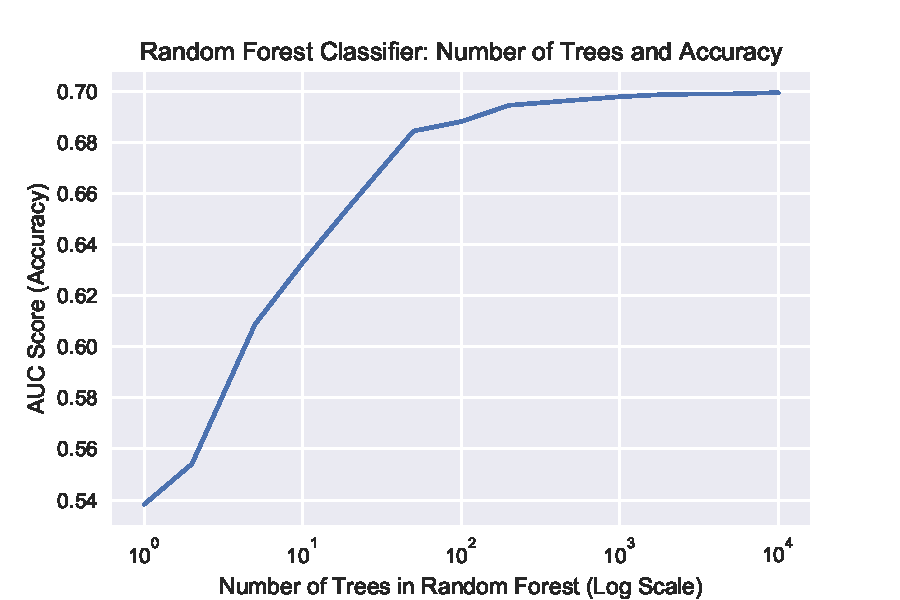
\includegraphics[width=\textwidth]{graphics/num_trees_rfc}
    \caption{Changes in classification accuracy (AUC score) as the number of trees in a random forest classification model are varied. The $x$-axis is on a log scale.}
    \label{fig:num_trees_rfc}
\end{figure}

\begin{figure}[!htbp]
    \centering
    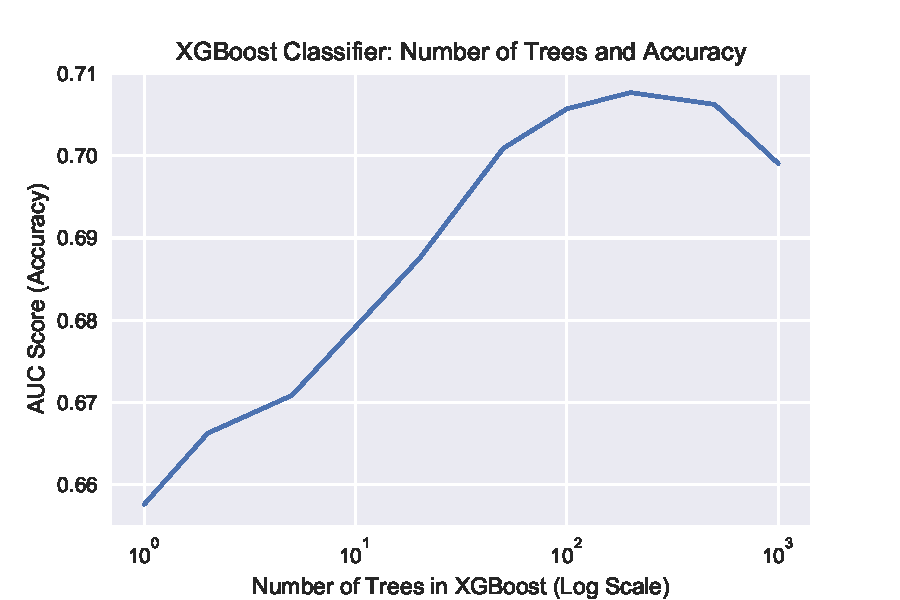
\includegraphics[width=\textwidth]{graphics/num_trees_xgbc}
    \caption{Changes in classification accuracy (AUC score) as the number of trees in a gradient tree boosting classification model are varied. The $x$-axis is on a log scale.}
    \label{fig:num_trees_xgbc}
\end{figure}

\subsection{Regression}

Again, since regression is the standard for econometric analysis, Table \ref{table:linear_results} contains the output for an ordinary least squares regression on the interest rate.

The variables discussed in Section \ref{subsection:classification_results} as having a negative impact on loan repayment probability also have a positive impact on interest rate. This observation is consistent with the fact that if investors are likely to lose money by not being repaid, then they will want to compensate by increasing the interest rate required for the loan. In addition, several other variables also positively impacted interest rate, suggesting that LendingClub takes these factors into account when assigning interest rates for loans.
Whereas \texttt{funded\_amount}, like the previously discussed variable \texttt{term}, is a reflection of loan size and therefore corresponds to a higher interest rate, increases in variables like \texttt{delinq\_2yrs} and \texttt{open\_accounts}, correspond to borrowers with higher risk of default; again, LendingClub must compensate by assigning a higher interest rate to these loans. Other interesting observations include the fact that a shorter credit history is associated with a higher interest rate, adjusting for the other variables; additionally, renting rather than owning a home is associated with a higher interest rate, perhaps because renting suggests less income stability than home ownership.

Variables that correspond to a significant negative impact on interest rate included \texttt{total\_accounts}, which typically corresponds to a longer credit history. Interestingly, there is a remarkable difference between \texttt{total\_accounts} and \texttt{open\_accounts}, which has a significant positive impact on interest rate. This discrepancy probably arises because an excess of open accounts suggests a large amount of credit, whereas a large number of total accounts (open and closed) suggests both responsibility in closing excess accounts and a longer credit history. Other important variables were \texttt{has\_employment}, which coincides with the intuition that employed borrowers are far less risky than unemployed borrowers and thus need a lower interest rate, and \texttt{issue\_year}, meaning that interest rates fell from 2007--2011. This second observation could arise from LendingClub becoming more lenient with interest rates since its inception or from interest rates around the world falling in the years after the financial crisis (and LendingClub following suit).

\begin{table}[!htbp]
    \footnotesize
    \begin{center}
\begin{tabular}{lclc}
\toprule
\textbf{Dep. Variable:}                        &     int\_rate     & \textbf{  R-squared:         } &     0.527   \\
\textbf{Model:}                                &       OLS        & \textbf{  Adj. R-squared:    } &     0.526   \\
\textbf{Method:}                               &  Least Squares   & \textbf{  F-statistic:       } &     893.8   \\
\textbf{Date:}                                 & Sun, 04 Mar 2018 & \textbf{  Prob (F-statistic):} &     0.00    \\
\textbf{Time:}                                 &     14:14:26     & \textbf{  Log-Likelihood:    } &   -70152.   \\
\textbf{No. Observations:}                     &       29754      & \textbf{  AIC:               } & 1.404e+05   \\
\textbf{Df Residuals:}                         &       29716      & \textbf{  BIC:               } & 1.407e+05   \\
\textbf{Df Model:}                             &          37      & \textbf{                     } &             \\
\bottomrule
\end{tabular}
\begin{tabular}{lcccccc}
                                               & \textbf{coef} & \textbf{std err} & \textbf{t} & \textbf{P$>|t|$} & \textbf{[0.025} & \textbf{0.975]}  \\
\midrule
\textbf{funded\_amnt}                          &       0.0001  &     2.61e-06     &    40.497  &         0.000        &        0.000    &        0.000     \\
\textbf{term}                                  &       0.1317  &        0.002     &    83.256  &         0.000        &        0.129    &        0.135     \\
\textbf{emp\_length}                           &      -0.0029  &        0.004     &    -0.657  &         0.511        &       -0.012    &        0.006     \\
\textbf{annual\_inc}                           &    8.286e-07  &     2.45e-07     &     3.386  &         0.001        &     3.49e-07    &     1.31e-06     \\
\textbf{dti}                                   &      -0.0111  &        0.003     &    -4.386  &         0.000        &       -0.016    &       -0.006     \\
\textbf{delinq\_2yrs}                          &       1.3195  &        0.029     &    45.481  &         0.000        &        1.263    &        1.376     \\
\textbf{inq\_last\_6mths}                      &       0.4117  &        0.010     &    40.796  &         0.000        &        0.392    &        0.431     \\
\textbf{open\_acc}                             &       0.1149  &        0.005     &    24.198  &         0.000        &        0.106    &        0.124     \\
\textbf{pub\_rec}                              &       0.9919  &        0.108     &     9.209  &         0.000        &        0.781    &        1.203     \\
\textbf{revol\_bal}                            &   -6.277e-06  &     8.06e-07     &    -7.791  &         0.000        &    -7.86e-06    &     -4.7e-06     \\
\textbf{revol\_util}                           &       0.0587  &        0.001     &    99.130  &         0.000        &        0.058    &        0.060     \\
\textbf{total\_acc}                            &      -0.0388  &        0.002     &   -19.783  &         0.000        &       -0.043    &       -0.035     \\
\textbf{pub\_rec\_bankruptcies}                &       0.1623  &        0.128     &     1.266  &         0.205        &       -0.089    &        0.414     \\
\textbf{tax\_liens}                            &      -2.8342  &        2.562     &    -1.106  &         0.269        &       -7.857    &        2.188     \\
\textbf{has\_employment}                       &    -139.8541  &        4.879     &   -28.666  &         0.000        &     -149.417    &     -130.291     \\
\textbf{issue\_month}                          &      -0.0304  &        0.004     &    -6.904  &         0.000        &       -0.039    &       -0.022     \\
\textbf{issue\_year}                           &      -0.4065  &        0.018     &   -23.001  &         0.000        &       -0.441    &       -0.372     \\
\textbf{earliest\_cr\_line\_month}             &      -0.0008  &        0.004     &    -0.187  &         0.851        &       -0.009    &        0.007     \\
\textbf{earliest\_cr\_line\_year}              &       0.0726  &        0.002     &    29.716  &         0.000        &        0.068    &        0.077     \\
\textbf{home\_ownership\_NONE}                 &      -0.7389  &        1.810     &    -0.408  &         0.683        &       -4.287    &        2.809     \\
\textbf{home\_ownership\_OTHER}                &       0.8945  &        0.260     &     3.443  &         0.001        &        0.385    &        1.404     \\
\textbf{home\_ownership\_OWN}                  &       0.5526  &        0.059     &     9.343  &         0.000        &        0.437    &        0.669     \\
\textbf{home\_ownership\_RENT}                 &       0.5026  &        0.035     &    14.283  &         0.000        &        0.434    &        0.572     \\
\textbf{purpose\_credit\_card}                 &       0.1809  &        0.089     &     2.036  &         0.042        &        0.007    &        0.355     \\
\textbf{purpose\_debt\_consolidation}          &       0.5820  &        0.082     &     7.132  &         0.000        &        0.422    &        0.742     \\
\textbf{purpose\_educational}                  &       1.1506  &        0.171     &     6.714  &         0.000        &        0.815    &        1.487     \\
\textbf{purpose\_home\_improvement}            &       0.7704  &        0.095     &     8.122  &         0.000        &        0.585    &        0.956     \\
\textbf{purpose\_house}                        &       1.0238  &        0.166     &     6.167  &         0.000        &        0.698    &        1.349     \\
\textbf{purpose\_major\_purchase}              &       0.6993  &        0.100     &     7.001  &         0.000        &        0.504    &        0.895     \\
\textbf{purpose\_medical}                      &       0.7445  &        0.137     &     5.425  &         0.000        &        0.475    &        1.013     \\
\textbf{purpose\_moving}                       &       0.8163  &        0.148     &     5.532  &         0.000        &        0.527    &        1.106     \\
\textbf{purpose\_other}                        &       0.9655  &        0.090     &    10.773  &         0.000        &        0.790    &        1.141     \\
\textbf{purpose\_renewable\_energy}            &       0.7278  &        0.320     &     2.276  &         0.023        &        0.101    &        1.354     \\
\textbf{purpose\_small\_business}              &       1.5591  &        0.104     &    14.967  &         0.000        &        1.355    &        1.763     \\
\textbf{purpose\_vacation}                     &       0.8691  &        0.170     &     5.115  &         0.000        &        0.536    &        1.202     \\
\textbf{purpose\_wedding}                      &       0.7929  &        0.123     &     6.426  &         0.000        &        0.551    &        1.035     \\
\textbf{verification\_status\_Source Verified} &       0.2282  &        0.040     &     5.724  &         0.000        &        0.150    &        0.306     \\
\textbf{verification\_status\_Verified}        &       0.4020  &        0.039     &    10.298  &         0.000        &        0.326    &        0.479     \\
\bottomrule
\end{tabular}
% \begin{tabular}{lclc}
% \textbf{Omnibus:}       & 634.792 & \textbf{  Durbin-Watson:     } &     1.995  \\
% \textbf{Prob(Omnibus):} &   0.000 & \textbf{  Jarque-Bera (JB):  } &   712.963  \\
% \textbf{Skew:}          &   0.327 & \textbf{  Prob(JB):          } & 1.52e-155  \\
% \textbf{Kurtosis:}      &   3.384 & \textbf{  Cond. No.          } &  3.22e+07  \\
% \bottomrule
% \end{tabular}
%\caption{OLS Regression Results}
\end{center}
    \caption{OLS regression results.}
    \label{table:linear_results}
\end{table}

Figures \ref{fig:regression_r2} and \ref{fig:regression_errors} contain visualizations of the regression models used in this paper. As in the classification setting, tree models performed significantly better than the corresponding regression, with XGBoost beating the random forest, which consistently beat extremely randomized trees. As in the classification case, I opted to add another model that takes the average prediction between the two best models, random forest and XGBoost, weighted by an accuracy score ($R^2$ for regression). This model outperformed both individual models. 

\begin{figure}[!htbp]
    \centering
    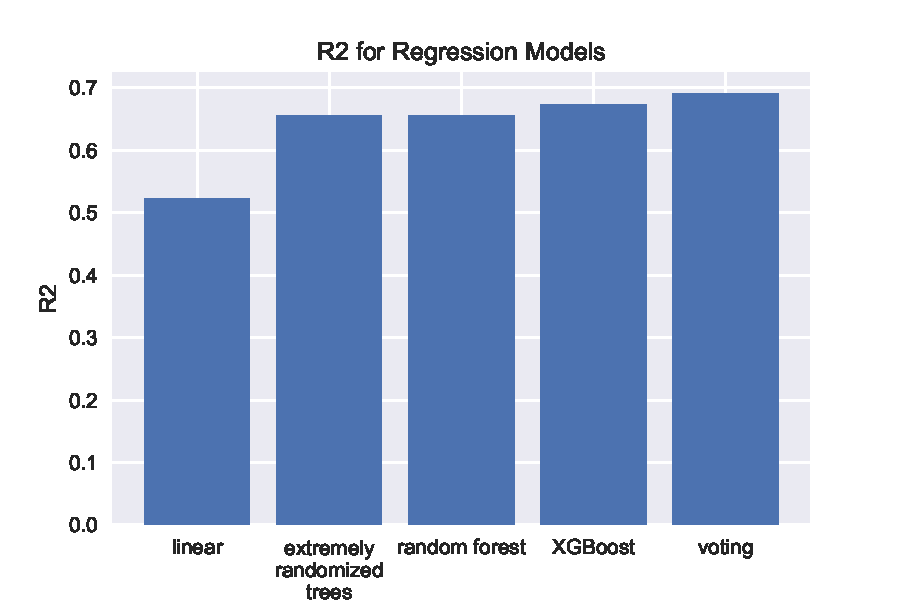
\includegraphics[width=\textwidth]{graphics/regression_r2}
    \caption{$R^2$ for regression models. An $R^2$ value of $0$ corresponds to no predictive power, and an $R^2$ value of $1$ corresponds to perfect predictive power.}
    \label{fig:regression_r2}
\end{figure}

\begin{figure}[!htbp]
    \centering
    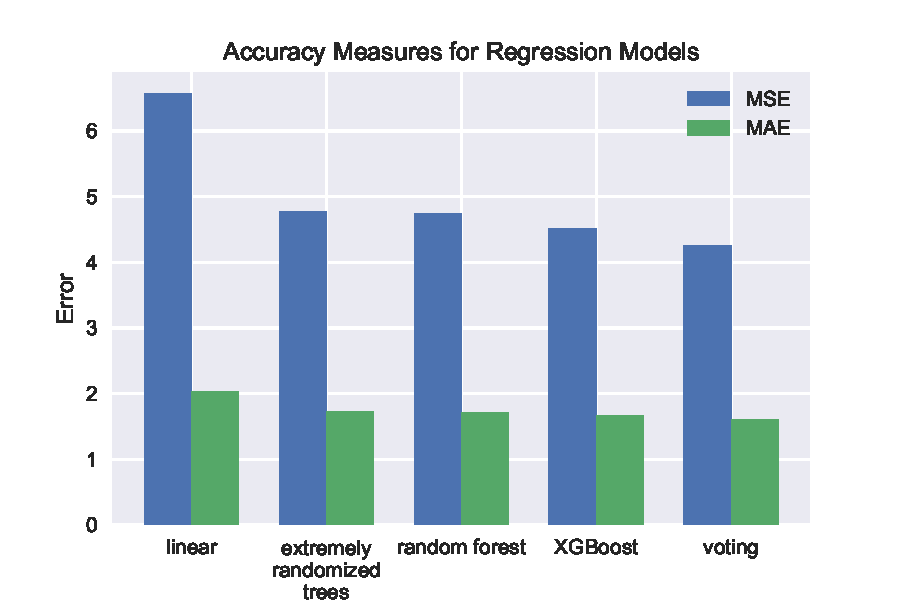
\includegraphics[width=\textwidth]{graphics/regression_errors}
    \caption{Two error types (mean squared error and mean absolute error) for regression models. Smaller values correspond to better models.}
    \label{fig:regression_errors}
\end{figure}

Interestingly, for predicting the interest rate, adding \texttt{installment} to the list of feature variables improved the $R^2$ of the XGBoost regressor to more than $0.99$, the mean squared error to about $0.13$. However, this addition did not significantly improve the accuracy of the other models. Because the monthly installment is a complex (though deterministic) function of the interest rate, the principal, and the term of the loan, this extraordinary accuracy suggests that the XGBoost model is particularly strong in modeling complex functions of the feature variables.

\subsubsection{Feature Importances}

Feature importances for regression models are defined in the same manner as for classification models. See Table \ref{table:regression_importances} for the feature importances for the best individual regression model, gradient tree boosting. The three variables most important in the classification setting (revolving balance, debt-to-income ratio, and annual income) also appear in the regression setting, followed by the loan amount and the borrower's revolving utilization. 

\begin{table}[!ht]
\footnotesize
\centering

\begin{tabular}{crc}
\toprule
\textbf{Rank} & \textbf{Variable} & \textbf{Feature Importance} \\ \midrule
1 & revol\_bal & 0.182871 \\
2 & dti & 0.138585 \\
3 & annual\_inc & 0.118966 \\
4 & revol\_util & 0.106197 \\
5 & funded\_amnt & 0.094184 \\
6 & total\_acc & 0.053128 \\
7 & earliest\_cr\_line\_year & 0.046728 \\
8 & open\_acc & 0.042176 \\
9 & issue\_month & 0.032825 \\
10 & earliest\_cr\_line\_month & 0.029596 \\
11 & emp\_length & 0.026586 \\
12 & inq\_last\_6mths & 0.021946 \\
13 & issue\_year & 0.020652 \\
14 & delinq\_2yrs & 0.009308 \\
15 & purpose\_debt\_consolidation & 0.008595 \\
16 & term & 0.008246 \\
17 & home\_ownership\_RENT & 0.005977 \\
18 & purpose\_credit\_card & 0.005192 \\
19 & purpose\_home\_improvement & 0.004683 \\
20 & purpose\_other & 0.004538 \\
21 & verification\_status\_Source Verified & 0.004159 \\
22 & purpose\_major\_purchase & 0.004058 \\
23 & pub\_rec & 0.004058 \\
24 & purpose\_small\_business & 0.003839 \\
25 & verification\_status\_Verified & 0.003767 \\
26 & purpose\_wedding & 0.002967 \\
27 & home\_ownership\_OWN & 0.002865 \\
28 & purpose\_house & 0.002225 \\
29 & purpose\_educational & 0.002109 \\
30 & pub\_rec\_bankruptcies & 0.002094 \\
31 & purpose\_medical & 0.001891 \\
32 & purpose\_vacation & 0.001658 \\
33 & purpose\_moving & 0.001600 \\
34 & purpose\_renewable\_energy & 0.000756 \\
35 & home\_ownership\_OTHER & 0.000494 \\
36 & home\_ownership\_NONE & 0.000335 \\
37 & tax\_liens & 0.000145 \\
38 & has\_employment & 0.000000 \\
\bottomrule
\end{tabular}
\caption{Variables ranked by feature importance for the best regression model tested (gradient tree boosting). Note that importance does not consider positive or negative influence, just absolute influence. }
\label{table:regression_importances}
\end{table}

\subsubsection{Hyperparameter Tuning}

As in the classification setting, I determined the relationship between accuracy (mean squared error for regression) and the number of trees included in the model for the two best models. Both models (Figures \ref{fig:num_trees_rfr} and \ref{fig:num_trees_xgbr}) show that after about 100 trees, increasing the number of trees results in very little improvement in accuracy. 

\begin{figure}[!htbp]
    \centering
    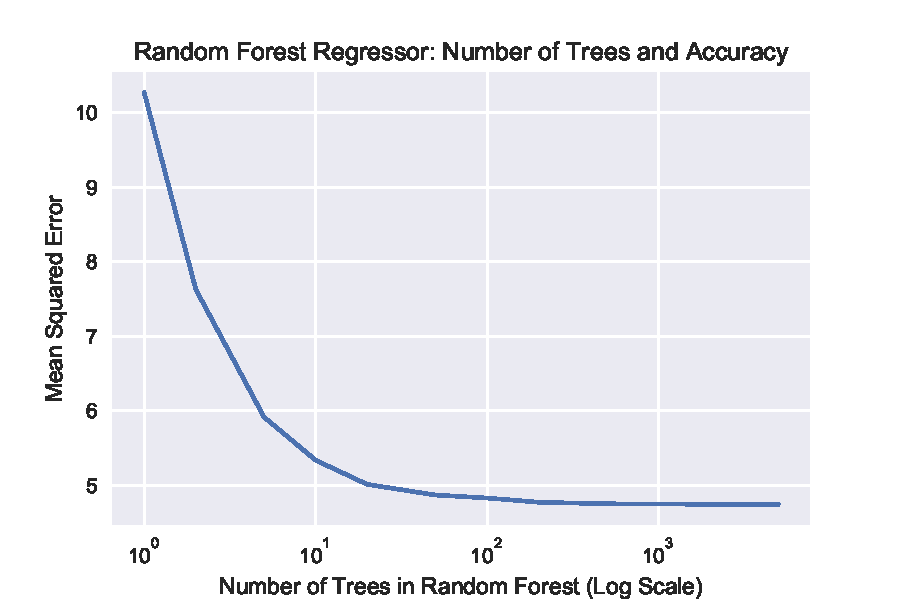
\includegraphics[width=\textwidth]{graphics/num_trees_rfr}
    \caption{Changes in regression error (mean squared error) as the number of trees in a random forest regression model are varied. The $x$-axis is on a log scale.}
    \label{fig:num_trees_rfr}
\end{figure}

\begin{figure}[!htbp]
    \centering
    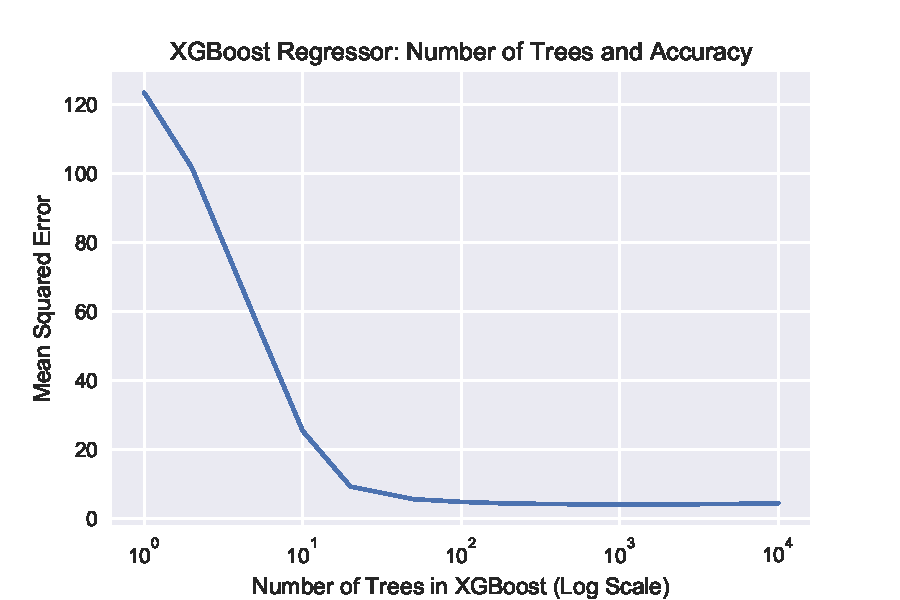
\includegraphics[width=\textwidth]{graphics/num_trees_xgbr}
    \caption{Changes in regression error (mean squared error) as the number of trees in a gradient tree boosting regression model are varied. The $x$-axis is on a log scale.}
    \label{fig:num_trees_xgbr}
\end{figure}

\section{Conclusion}

This paper explored the accuracy of simple regressions, neural networks, and several tree models in predicting loan repayment and assigned interest rate for a dataset of LendingClub loans between 2007--2011. I find that of the models considered, gradient tree boosting (XGBoost) performed the best. Moreover, tree models performed significantly better for both classification and regression than the corresponding logistic and linear regression models. I also find that measures of financial responsibility and length of credit history correlate positively with loan repayment probability and negatively with assigned interest rate. Measures of loan size, such as the loan amount and the term, have the opposite effect. 

\subsection{Further Direction}

One potential further direction involves incorporating LendingClub loans created after 2011, when LendingClub increased significantly in popularity. Investigating the effect of this increase in popularity on LendingClub's lending criteron as well as other time related-effects could result in new insights, particularly about LendingClub's internal interest rate determination algorithm and about changing borrowing habits. Additionally, using loan repayment predictions to manually optimize investors' portfolios and maximize returns can make LendingClub more efficient and a more attractive place to invest. 

\newpage
\bibliography{project}{}
\bibliographystyle{plain}

% https://stats.stackexchange.com/questions/162162/relative-variable-importance-for-boosting

% https://statistics.berkeley.edu/sites/default/files/tech-reports/666.pdf

% \url{https://github.com/ragraw26/Machine-Learning-Loan-Lending-Club/blob/master/Regression%20%26%20Classification/Classification_Assignment2.ipynb}: \url{http://scikit-learn.org/stable/modules/generated/sklearn.feature_selection.RFE.html}

% https://pdfs.semanticscholar.org/41fd/c40fc6cc1102ef8f0866e4196c8da831b151.pdf

% \url{https://scholar.google.com/scholar?hl=en&as_sdt=1%2C22&as_vis=1&q=machine+learning+%2B%22lendingclub%22+filetype%3Apdf}

\newpage
\appendix

\section{Code}
\label{appendix:code}

\singlespacing
\footnotesize
\python{lendingclub.py}

\end{document}